\documentclass{article}
\usepackage[utf8]{inputenc}

\title{TurtleBot Maze Solver}
\author{Tanay Nistala, Stephanie Wilson, Iris Yang}
\date{\vspace{-1em}}

\usepackage{natbib}
\usepackage{graphicx}
\usepackage{multicol}
\usepackage{multirow}
\usepackage{amsmath}

\begin{document}

\maketitle


\section{Introduction}


In the field of robotics, maze solution by a robot is an interesting challenge because of the localization and path finding algorithms used to perform it. This specific application of path finding and localization can be used for finding the best ways for a robot to navigate a space efficiently and safely, and has been used for the development of many path finding algorithms. Dynamic robot path finding that adapts to obstacles in surroundings can be used for many useful tasks for robots, like finding its way through unknown areas of people or difficult terrain. Robots that conduct tours, scout out areas unreachable by people, and map out terrain can all use algorithms like these to gather information more effectively. 


We propose to test several different established methods of localization and path finding of a Turtlebot simulation on different mazes that we generate. This will require fine-tuning of said methods to allow the Turtlebot to expertly navigate the mazes, and we will compare how fast they are able to localize and navigate the maze. Our results will provide more insight into how robots map out unknown areas, hopefully leading to future advancements in localization and path-finding algorithms. 



\section{Background Related Work}

When talking about the advancements in the robotics field, there are three potential pathways that have been developed upon in previous work. First is localization algorithms, and second is SLAM (Simultaneous Localization and Mapping) algorithms, and lastly there are path-finding algorithms. There are numerous works on many of these and how they have been developed. Our primary focus for the maze solving is how each of these three algorithms work together for the best results. 

\subsection{Robot Localization and SLAM Algorithms}

% Robot Localization & SLAM Algorithms 
% Yarovoi 2024
% Turnage 2016
% Cherubini 2014

For Robot localization algorithms, many advances have been made to the optimization of robots in different contexts. In Cherubini 2014, autonomous robot navigation is investigated using visual sensors for a robot to navigate a dynamic environment. This is based on a different framework, however, than the one we will be working with. Turnage 2016 tests the performance of different SLAM Algorithms, CoreSLAM, Gmapping, and HectorSLAM. The distances of the paths taken with each of the algorithms is compared on a 2D simulator, similar to our simulation of the Turtlebot3. Overall, this paper helps us make hypotheses about how the robot will perform with different algorithms in different environments, which varied in the results of this study. Finally, a paper by Yarovoi 2024 details the different techniques used for these SLAM algorithms, as a full general overview of the subject.


\subsection{Path-finding}

% Pathfinding
% Abiyev 2017
% Sang 2024
% Lai 2023

Several path-finding algorithms have been developed in the past. Numerous improvements have been made in the field to path-finding algorithms, and many are developed for certain situations. In Abiyev 2017, the A*, Rapidly Exploring Random Tree (RRT), and artificial potential field (APF) Algorithms are implemented into a Nao robot to see how well it would perform in an environment with many obstacles. An accurate map using the robot's camera was used, to focus solely on the path-finding algorithm's effectiveness in the study. In the study, they were able to find the effectiveness of the A* algorithm for vision based robotics, where other sensors may not be available or noisy. 

One algorithm, the Dynamic Window Algorithm (DWA), which was used for Turtlebot3's simulations, is examined in Lai 2023's paper for path planning. Lai proposed an enhanced version of this algorithm that focuses on smoother movements for the robot and more reasonable planning. The original DWA algorithm focuses on velocity sampling, and suffers when obstacles are dynamic. However, techniques have been made to allow the DWA algorithm to dynamically change its parameters based on the dynamic obstacles for better performance. This makes DWA much more dynamic to situations than other algorithms before. 

Another paper by Sang et al. 2024 proposed an approach that combines both the A* and DWA algorithms for robot path-finding. In the paper, they smoothen out the A* algorithm's paths using grids and reducing the number of turning points. Additionally, they improve upon the DWA algorithm by accounting for unknown obstacles in the algorithm's evaluation function. The paper then proposes a hybrid algorithm of A* and DWA. While A* makes an optimal path using what it knows, it lacks the capability to avoid unknown and moving obstacles. However, DWA can avoid unknown obstacles but the path it
generates is not optimal. Combining the two results in a solid algorithm for situations with unknown obstacles, just like in our mazes for our experiments.

\subsection{Applications to Turtlebot3 Simulation}

% Turtlebot application
% Thale 2020

In our project, we use the Turtlebot to accomplish these objectives. Thale et. al 2020 goes into the details of various SLAM algorithms used with ROS and the Turtlebot framework. We used their work and this paper as a guide for our project and experiments. Throughout the paper they detail simulating a mobile robot capable of visually detecting and
avoiding static obstacles using SLAM and reaching the desired
location autonomously. In the paper, they primarily use Gmapping SLAM with a particle filter for localization. We sought to evaluate the different approaches, but testing with other algorithms, to accomplishing this with the Turtlebot3 framework and simulation, detailed in the coming sections. 

\section{Approach}

For a robot to traverse a maze (or any environment, for that matter), it typically requires a map of said environment either as a physical map or some form of costmap, which can then be used for pathfinding. However, in this scenario no such map is made available to the robot. 

Producing a map of the environment is possible with the right sensor data and odometry, and simultaneous localization and mapping (SLAM) algorithms provide a means of doing so while also allowing the robot to localize itself within the unfamiliar environment. A similar issue is raised here, however, as these algorithms typically require manual teleoperated control through the unknown environment in order to build the map for future use. 

This creates a dilemma: traversing an environment autonomously requires a previously prepared map, which can itself only be produced through manual navigation. However, the modular framework provided by the Robot Operating System (ROS) lends itself well to the approach devised for solving this problem. For this maze solver, separate nodes can be initialized for navigation and SLAM, wherein the former "disguises" itself as a manual controller for the robot, while using odometry data published by the latter concurrently.

Further sections explain the setup of such a system in greater detail.

\subsection{Sensor Data and Odometry}

Sensor data and odometry are crucial for the localization of the robot, as this forms the base of reliability for future steps of this maze solver. Robust localization leads to more trustworthy data for mapping within the SLAM node, which in turn increases the accuracy of odometry passed on to the navigation node. Two main data sources are used for this: raw positional odometry from the robot's drive base, and LIDAR scanner measurements. 

The robot's drive base continually computes estimates the current position and pose (heading) from a calibrated base point (which is typically the point of initialization). This utilizes known data about the size of the robot's wheels along with the drive motors' operating speeds:
$$
\begin{aligned}
    \mathbf{v} &= \begin{bmatrix} v_{l} \\ v_{r} \end{bmatrix} \\
    \mathbf{w} &= \frac{1}{r_{wheel}} \mathbf{v} \\
    \mathbf{w}_{wheel} = \begin{bmatrix} w_{l} \\ w_{r} \end{bmatrix} &= \delta_t \mathbf{w} = \frac{\delta_t}{r_{wheel}} \mathbf{v} \\
    \delta_{s} &= r_{wheel} \frac{w_l + w_r}{2} \\
    \delta_{\theta} &= r_{wheel} \frac{w_r - w_l}{\delta_{wheel}}
\end{aligned}
$$


where $\delta_{wheel}$ is the separation between the robot's wheels.

LIDAR scans provides distance estimates to nearby obstacles in the environment. For simplicity, this is implemented as three laser beams: one directly ahead (0°), and two offset to the left and right (30° and -30°-330°). Since the LIDAR scanner rotates as it publishes data, this produces a 360° map of the environment from the robot's position; the main caveat here is that LIDAR sensors have a maximum range of measurements, resulting in limited data in large environments.

\subsection{Navigation}
Navigation is achieved through the dynamic window approach (DWA) method [@Fox1997], and is provided wholesale as part of TurtleBot's navigation libraries. This algorithm plans paths based on the available world map; for known areas of the map it can plan paths that avoid walls and obstacles between the robot and the destination, but plans a direct path to the destination in unknown areas of the map, lacking any data about the environment there. This algorithm takes into account the robot's own motion dynamics, such as turn radius and speed/acceleration. This allows for far more accurate path planning, and results in fewer instances of the robot getting itself stuck in tight spaces.

\subsection{SLAM}
SLAM algorithms bridge the gap between odometry and the navigation layer of the system, providing a means for interpreting the former to create a map for the latter. Odometry and LIDAR scans published by their respective nodes are consumed by the SLAM algorithm, which uses prior data about the environment and the robot's pose to localize the robot and potentially expand the internally generated map. In turn, the robot's (estimated) location and the map are published by the SLAM node for use by the navigation layer described above.

SLAM itself faces a similar problem experienced here with regards to the interdependence of multiple variables. For localization, an accurate and consistent map is required, but for mapping an accurate location is needed. Three main SLAM algorithms are utilized here as they are packaged within the ROS framework's SLAM module; each uses various sources of data: GMapping, Hector, and Karto. 

GMapping [@Grisetti2005] [@Grisetti2007], is one of the most accurate methods available for solving the SLAM problem, and utilizes a Rao-Blackwellized particle filter where each particle contains a separate map of the environment. Crucially, it relies on both robot odometry and LIDAR scans, which helps it achieve a high level of accuracy, but is still more tolerant of noise in the robot's motion model and sensors as compared to an Extended Kalman filter (EKF).

Hector [@Kohlbrecher2011], and uses an EKF instead. Designed to be much faster to process, it relies heavily on LIDAR data as odometry is optional. Localization is achieved through comparisons with nearby features, but requires little noise in sensor data and motion estimates. As such, it is more tolerant of drops in the odometry data stream, but typically this comes with a tradeoff in that the robot's motion must remain slow and controlled to avoid losing reference points too quickly.

Karto [@Konolige2010], achieves a balance between the aforementioned methods using a method called Sparse Pose Adjustment (SPA) that optimizes pose graphs. Importantly, it is tolerant of failure of odometry, unlike Hector; when lacking odometry data it can still generate consistent SLAM poses.

These three methods do create generally accurate maps of the robot's environment, but here we aim to investigate the effect of the SLAM method used on the robot's ability to autonomously navigate a new environment in addition to mapping it.

We are using Gazebo to visualize the mazes that the Turtlebot will be attempting to solve, as well as Rviz to log sensor data from the robot's sensors and measure how well it reaches its goal. 

\section{Experiment}

We wanted to do an experiment on how SLAM algorithms would quickly and efficiently let the Turtlebot traverse several mazes, which would hopefully give us an insight on where future research and/or improvements could be done on real Turtlebots to map out unknown locations swiftly. 

Instead of just using GMapping, as previous papers have done, we are also using Hector and Karto. Each algorithm will be run on each of the three mazes below in order to get an accurate representation of each of the SLAM algorithms in different contexts. Below are pictures of the three mazes, shown in Gazebo:

\begin{figure}[htbp]
    \centering
    \begin{minipage}{0.3\textwidth}
        \centering
        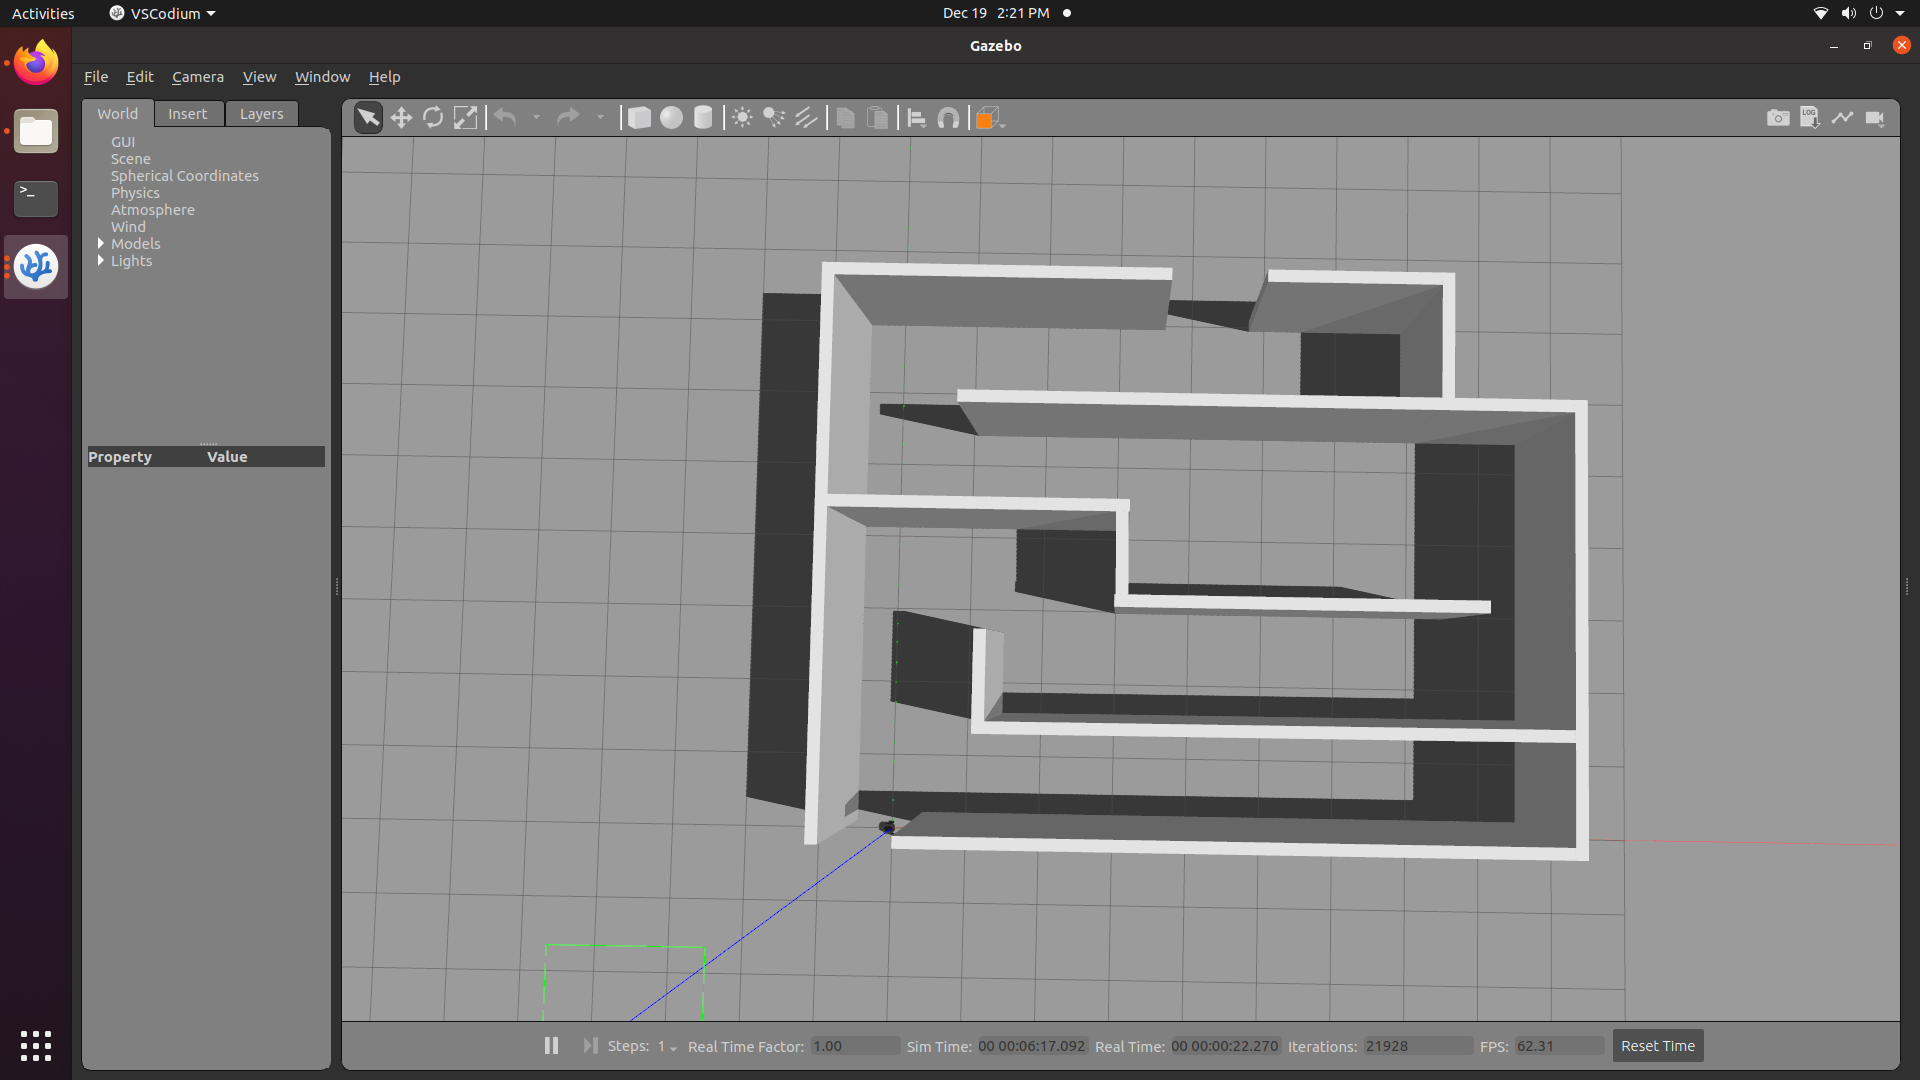
\includegraphics[width=\linewidth]{maze_1.png} 
        \caption{Maze 1}
    \end{minipage}%
    \hfill
    \begin{minipage}{0.3\textwidth}
        \centering
        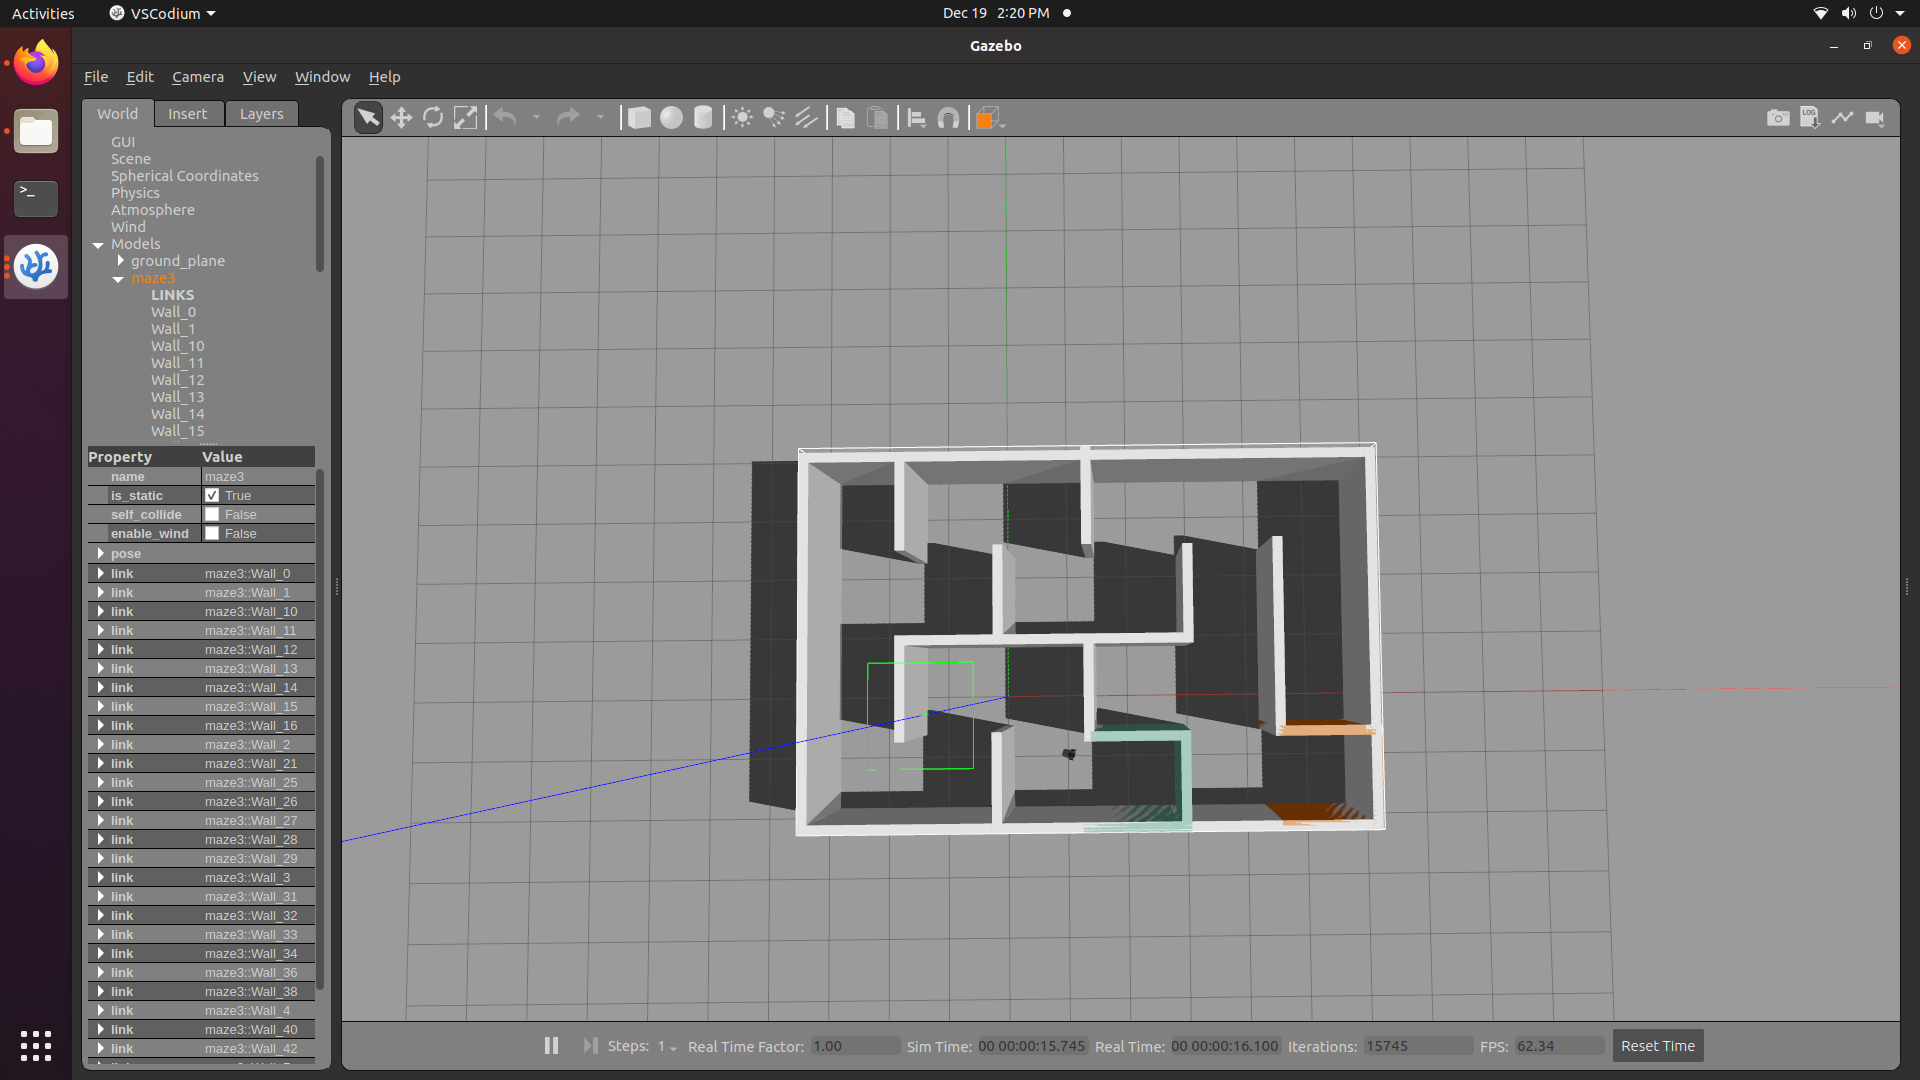
\includegraphics[width=\linewidth]{maze_3.png}
        \caption{Maze 3}
    \end{minipage}%
    \hfill
    \begin{minipage}{0.3\textwidth}
        \centering
        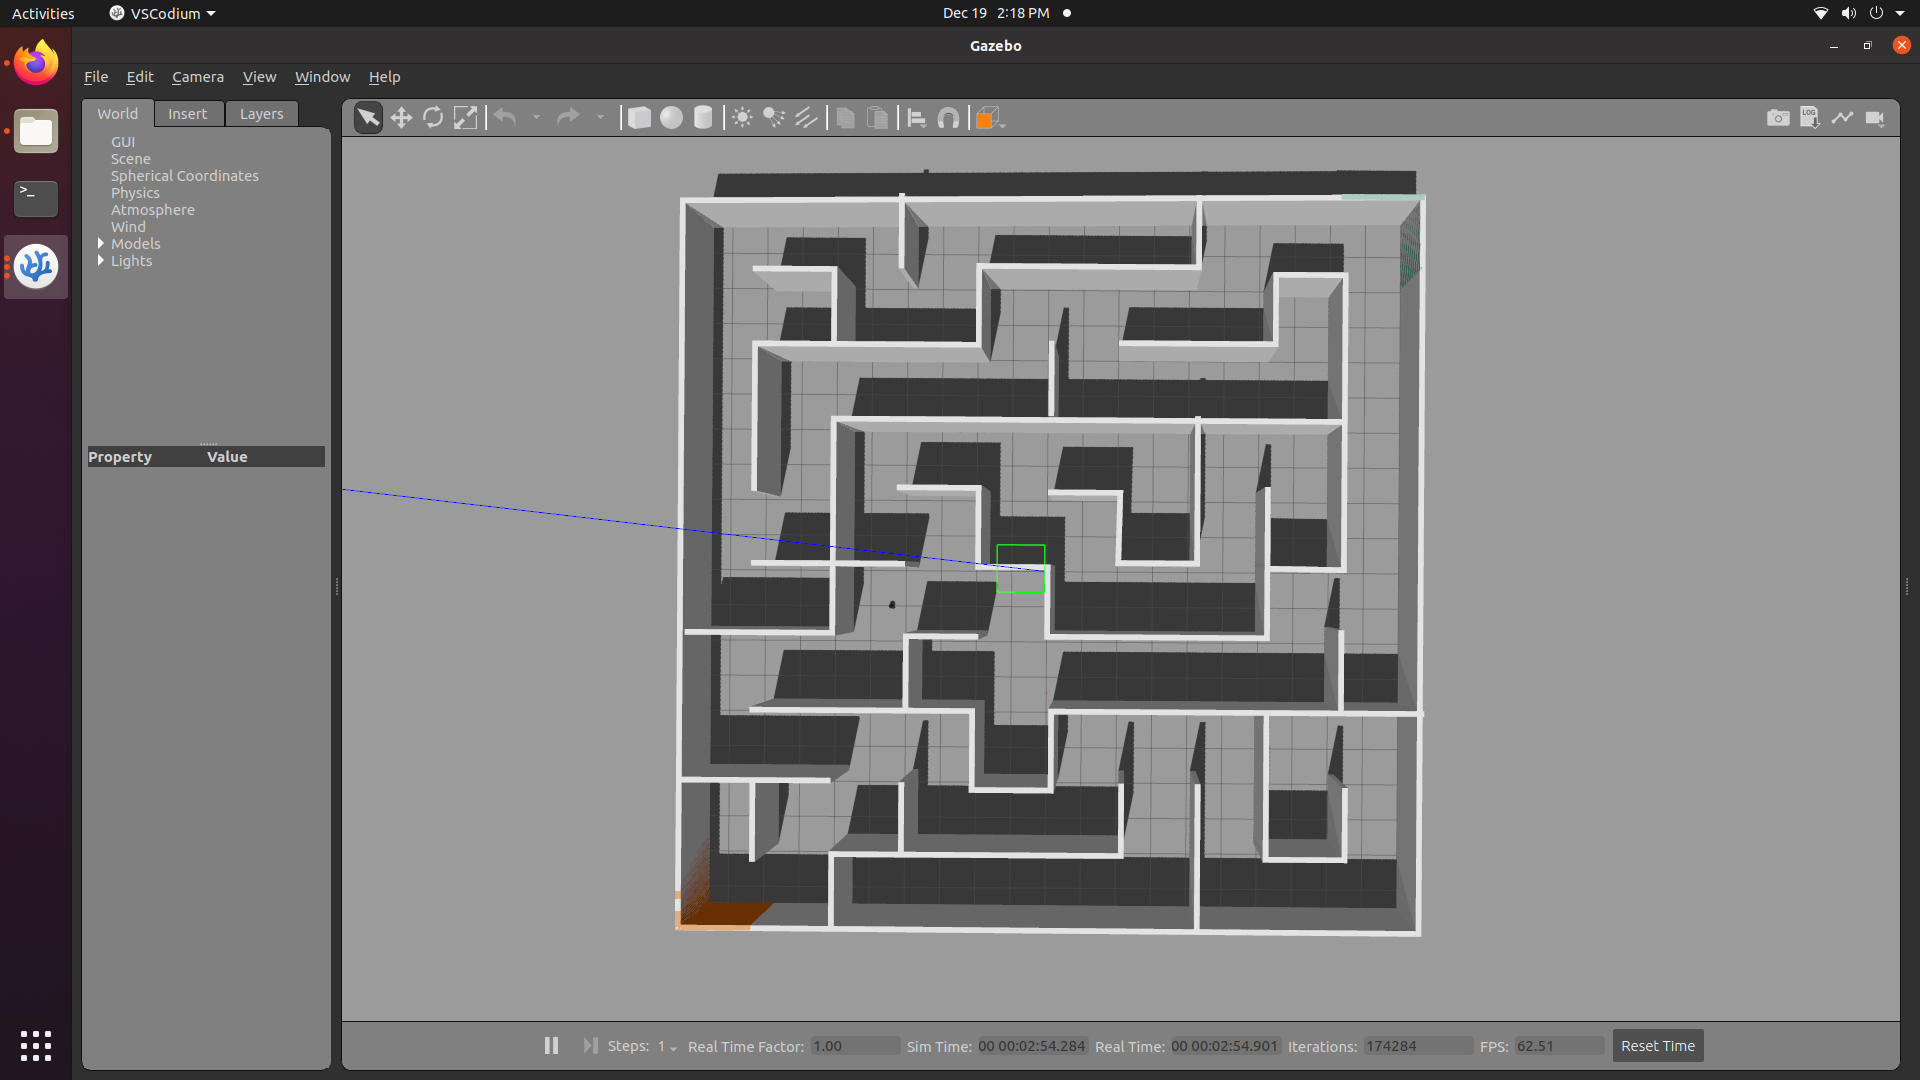
\includegraphics[width=\linewidth]{maze_4.png}
        \caption{Maze 4}
    \end{minipage}
\end{figure}

\subsection{Results}
After making the mazes, we launched the script in ROS, set the goal in Rviz for the Turtlebot to navigate to, and timed each run. 
In addition to the time it took to run through the maze, the map that each of the SLAM algorithms generated is reported. 

{\bf Maze 3, GMapping:}

\begin{figure}[htbp]
    \centering
    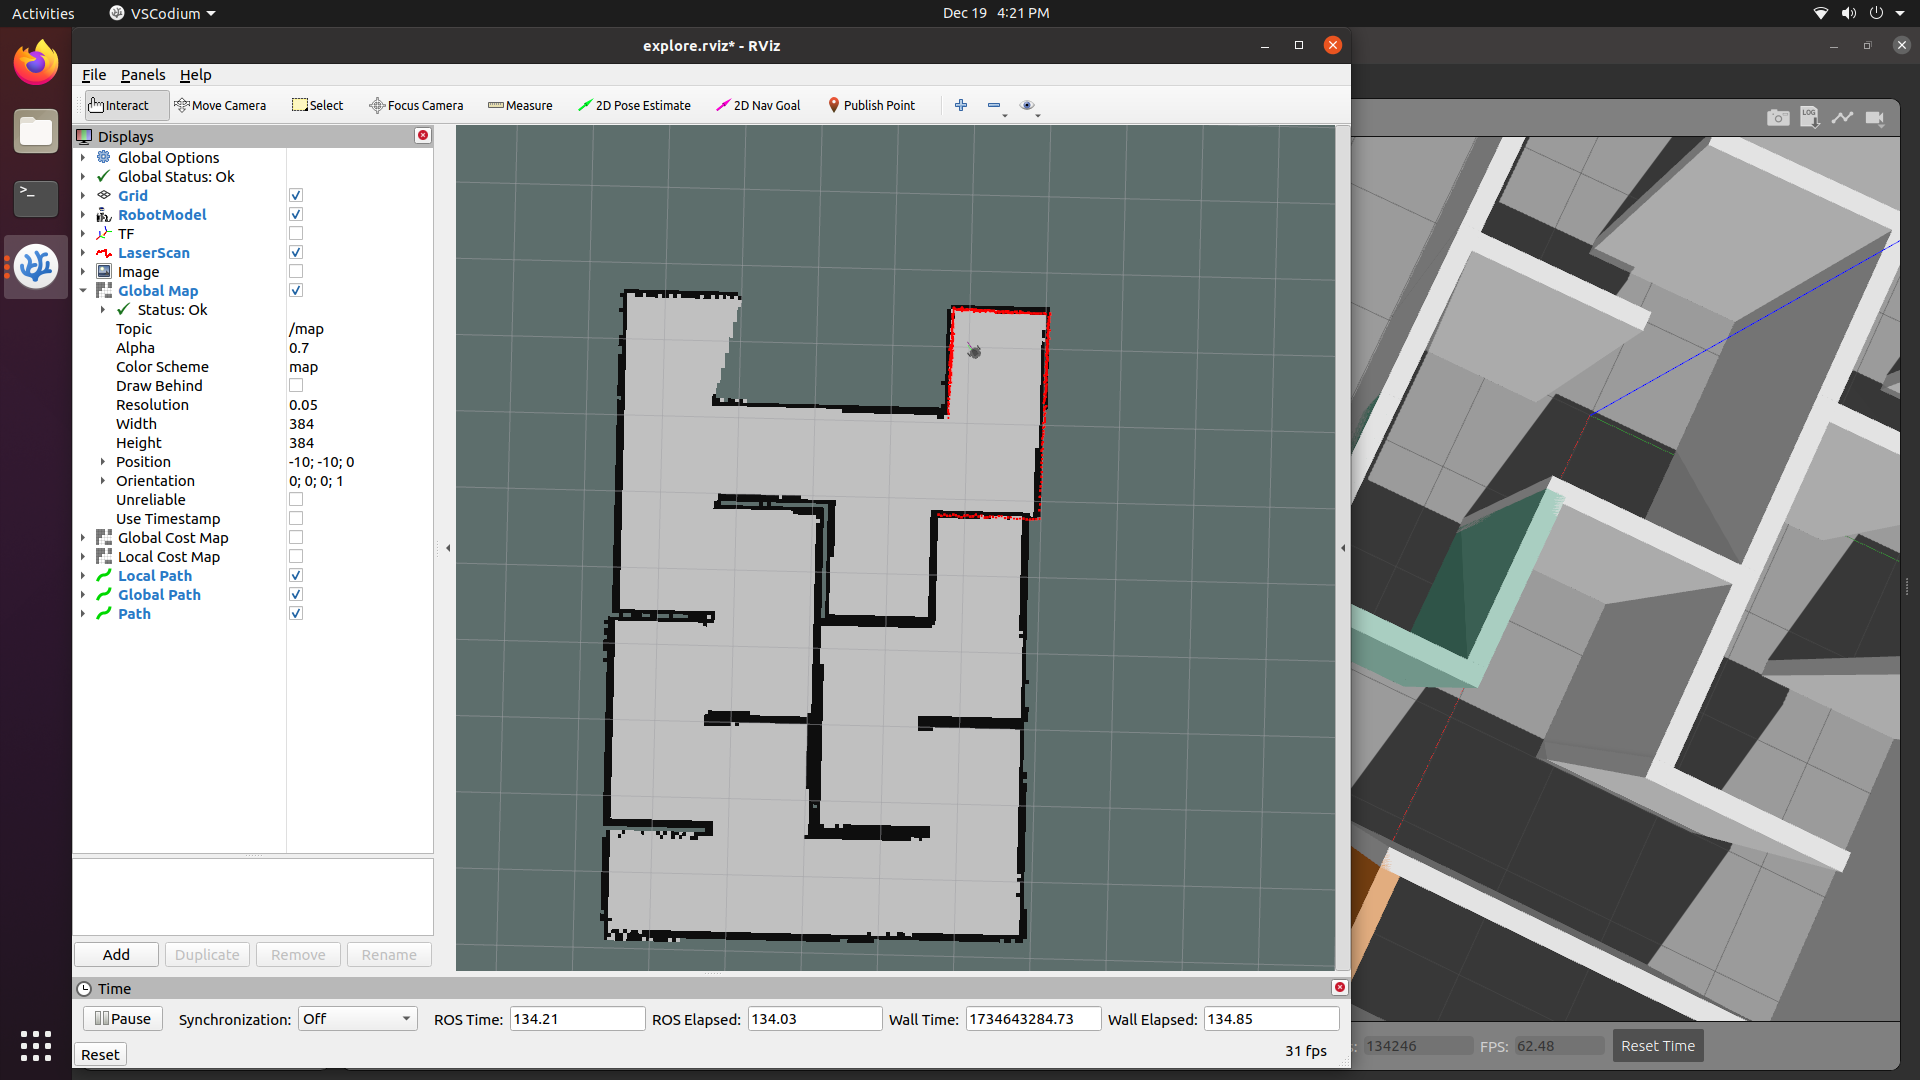
\includegraphics[width=\linewidth]{maze_3_gmapping.png} 
\end{figure}
\pagebreak
{\bf Maze 3, Hector:}

\begin{figure}[htbp]
    \centering
    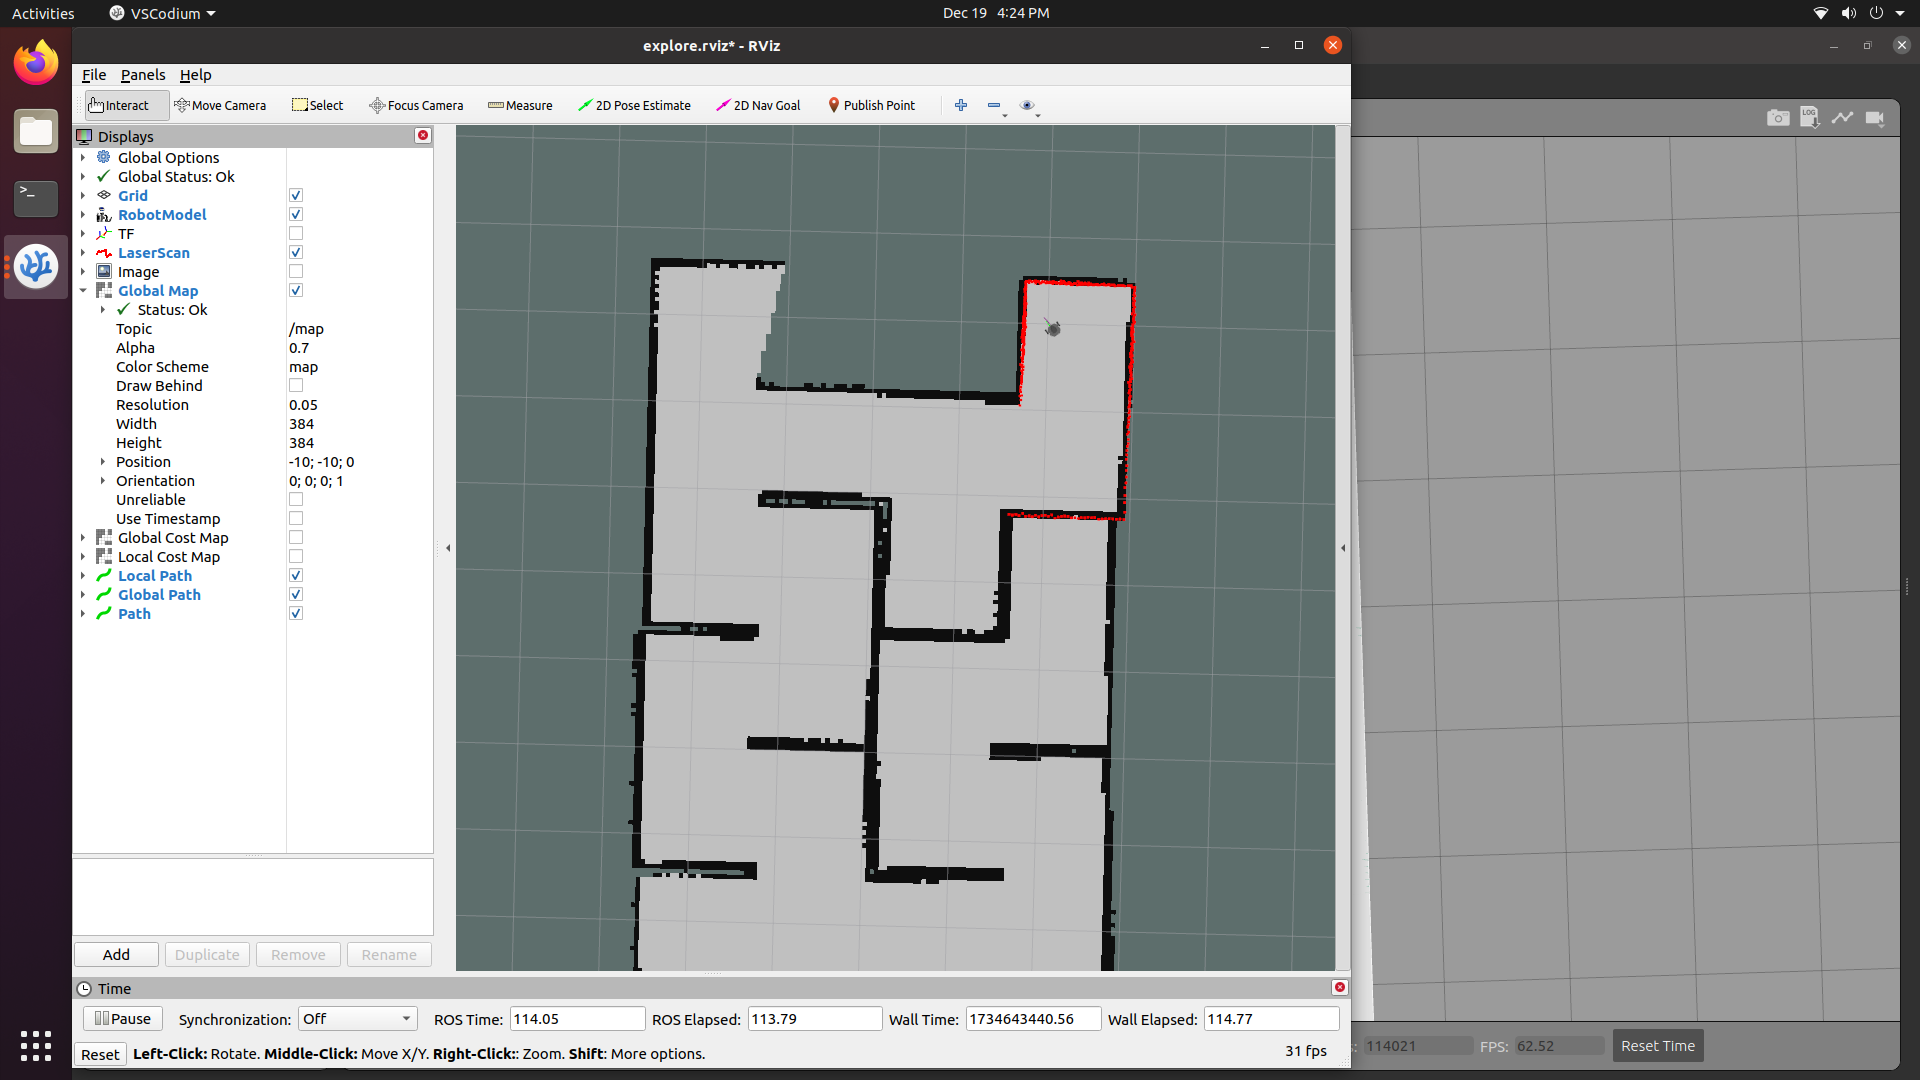
\includegraphics[width=\linewidth]{maze_3_hector.png} 
\end{figure}

{\bf Maze 3, Karto:}

\begin{figure}[htbp]
    \centering
    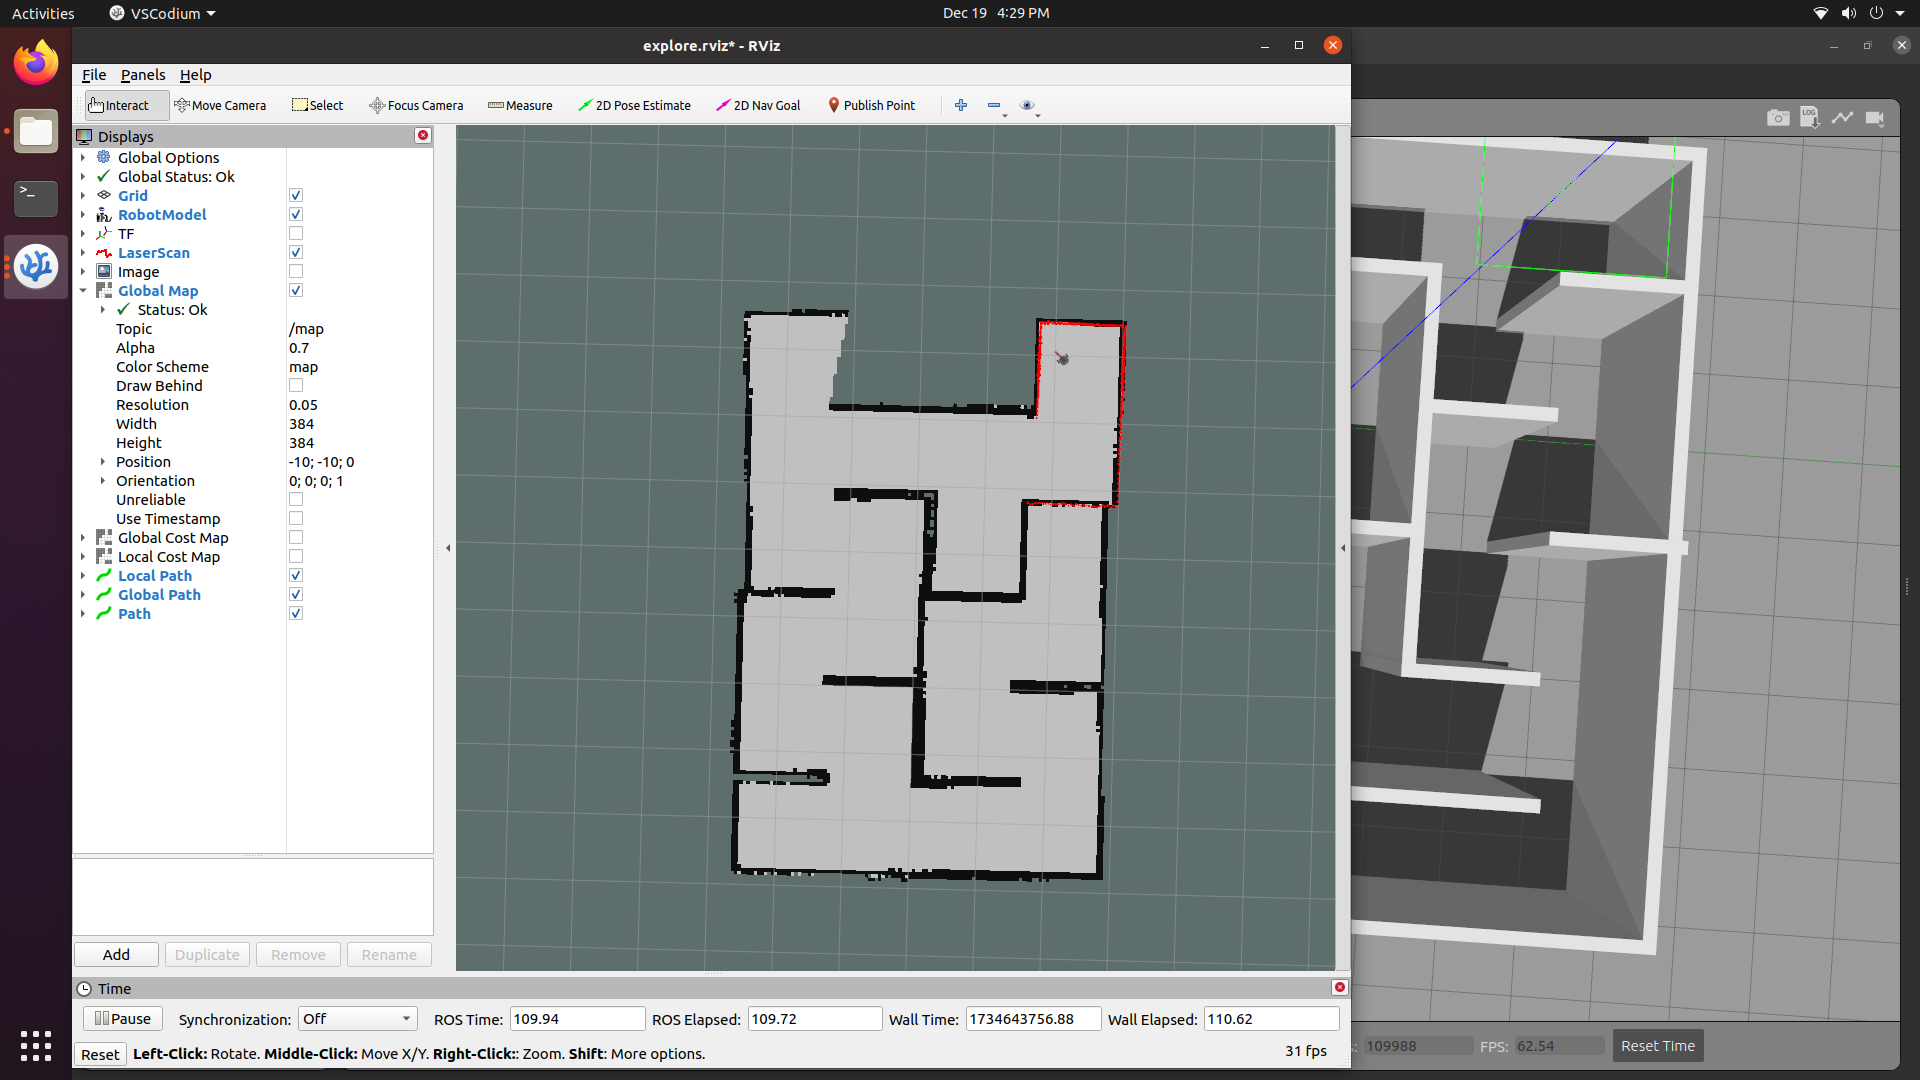
\includegraphics[width=\linewidth]{maze_3_karto.png} 
\end{figure}
\pagebreak
{\bf Maze 4, GMapping:}

\begin{figure}[htbp]
    \centering
    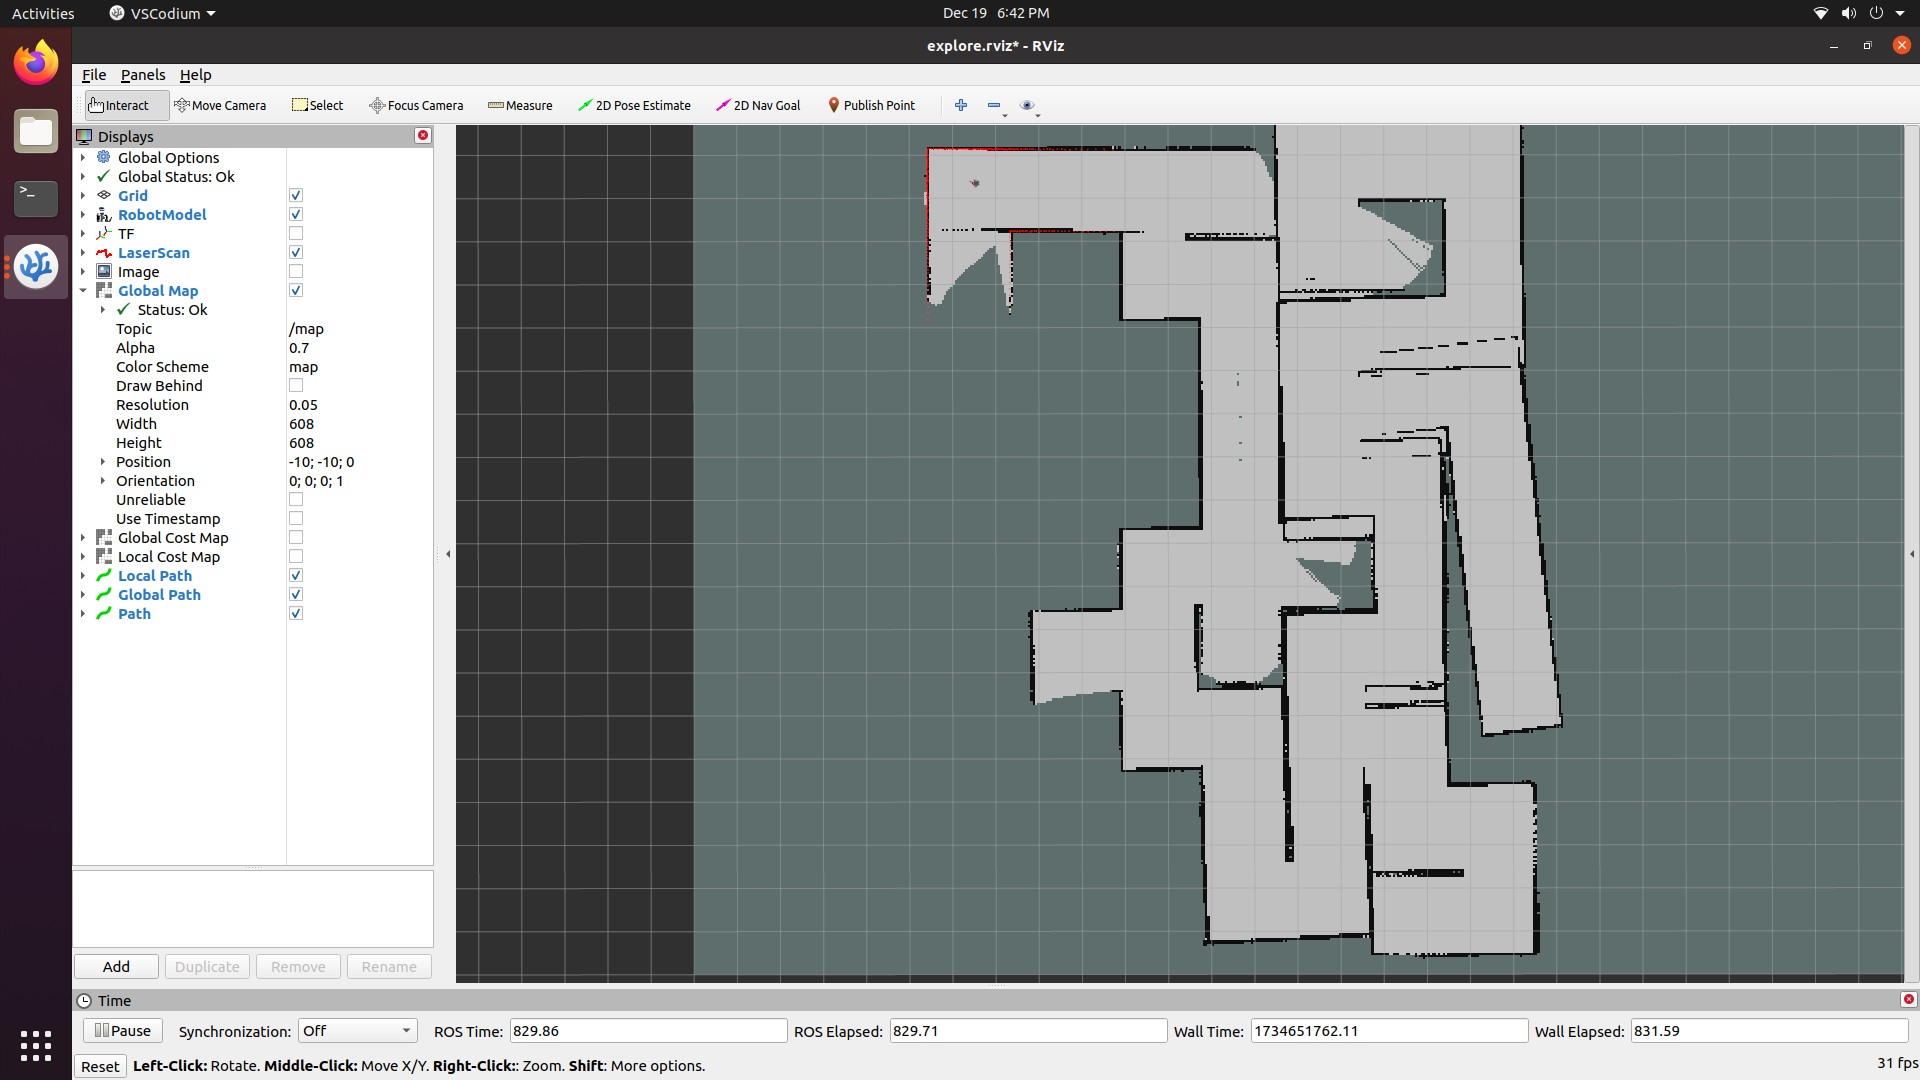
\includegraphics[width=\linewidth]{maze_4_gmapping.png} 
\end{figure}
{\bf Maze 4, Hector:}

\begin{figure}[htbp]
    \centering
    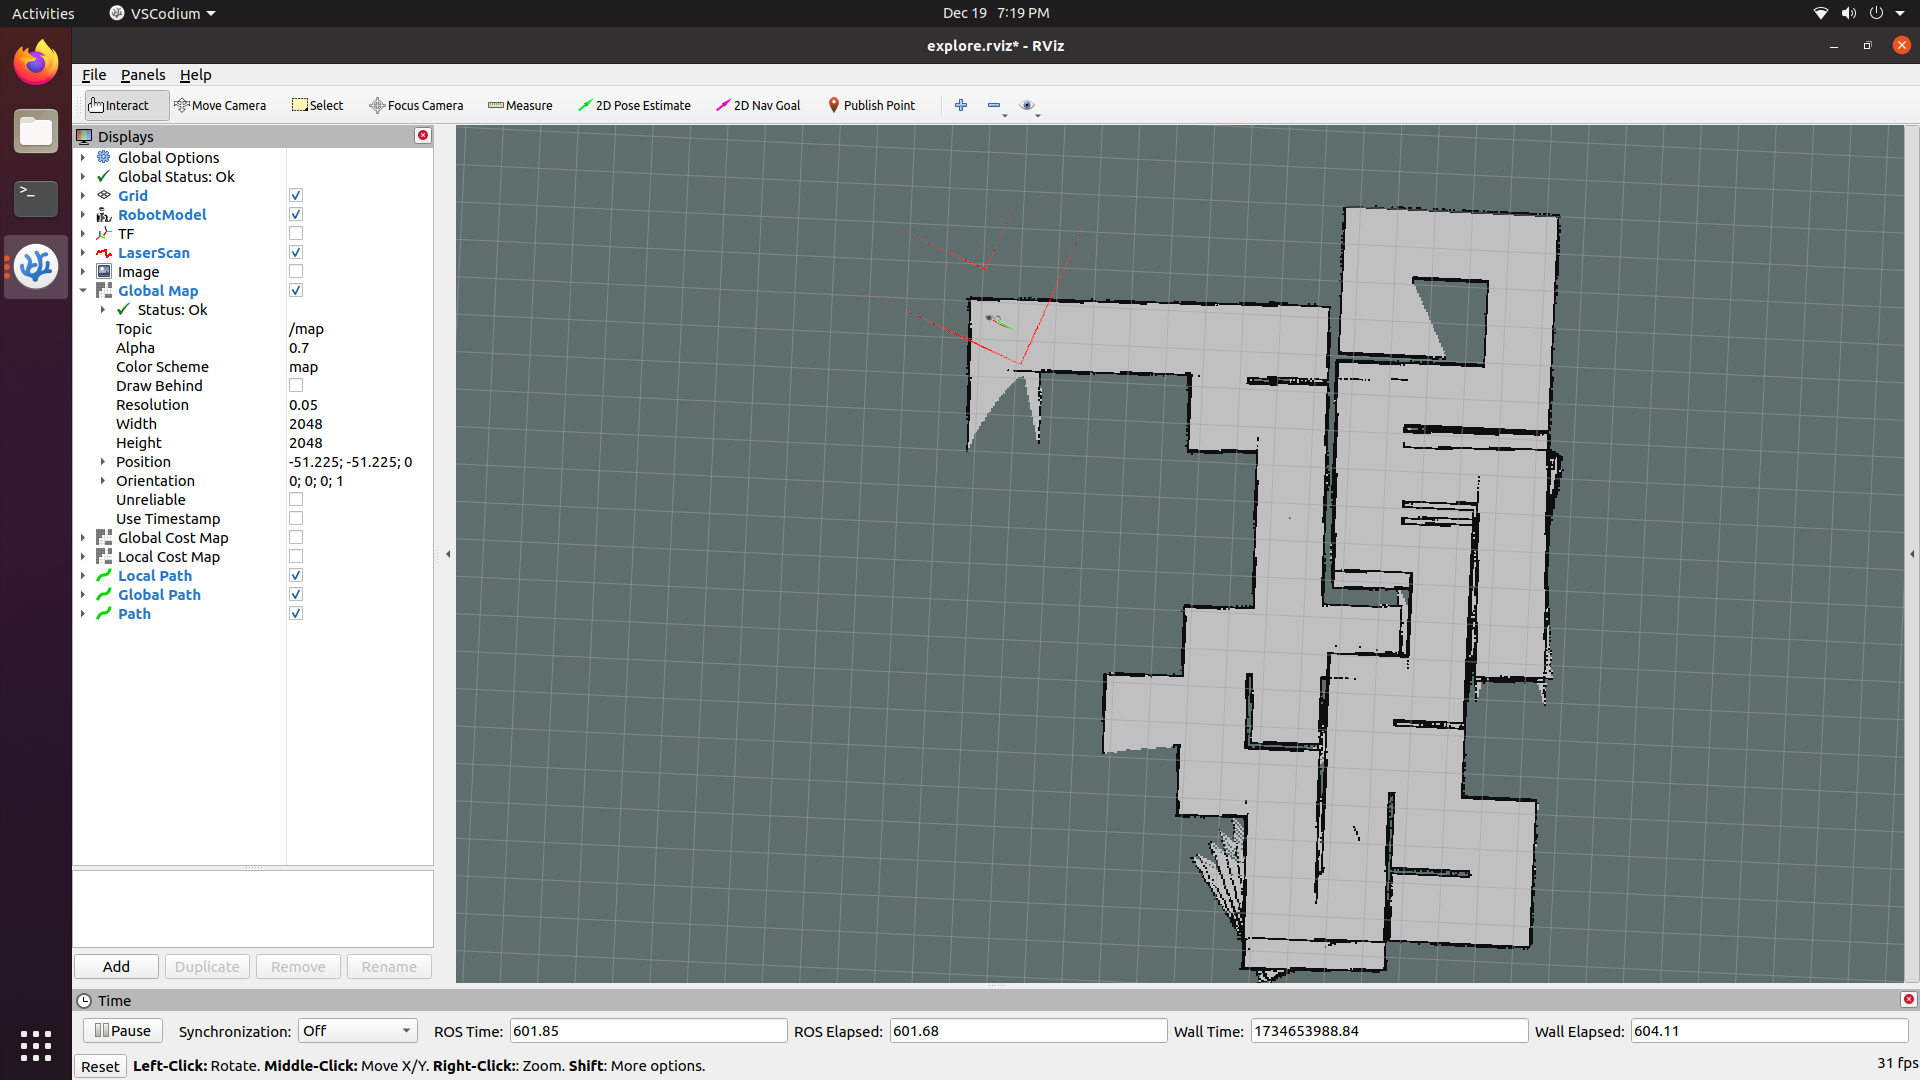
\includegraphics[width=\linewidth]{maze_4_hector.png} 
\end{figure}
\pagebreak
{\bf Maze 4, Karto:}

\begin{figure}[htbp]
    \centering
    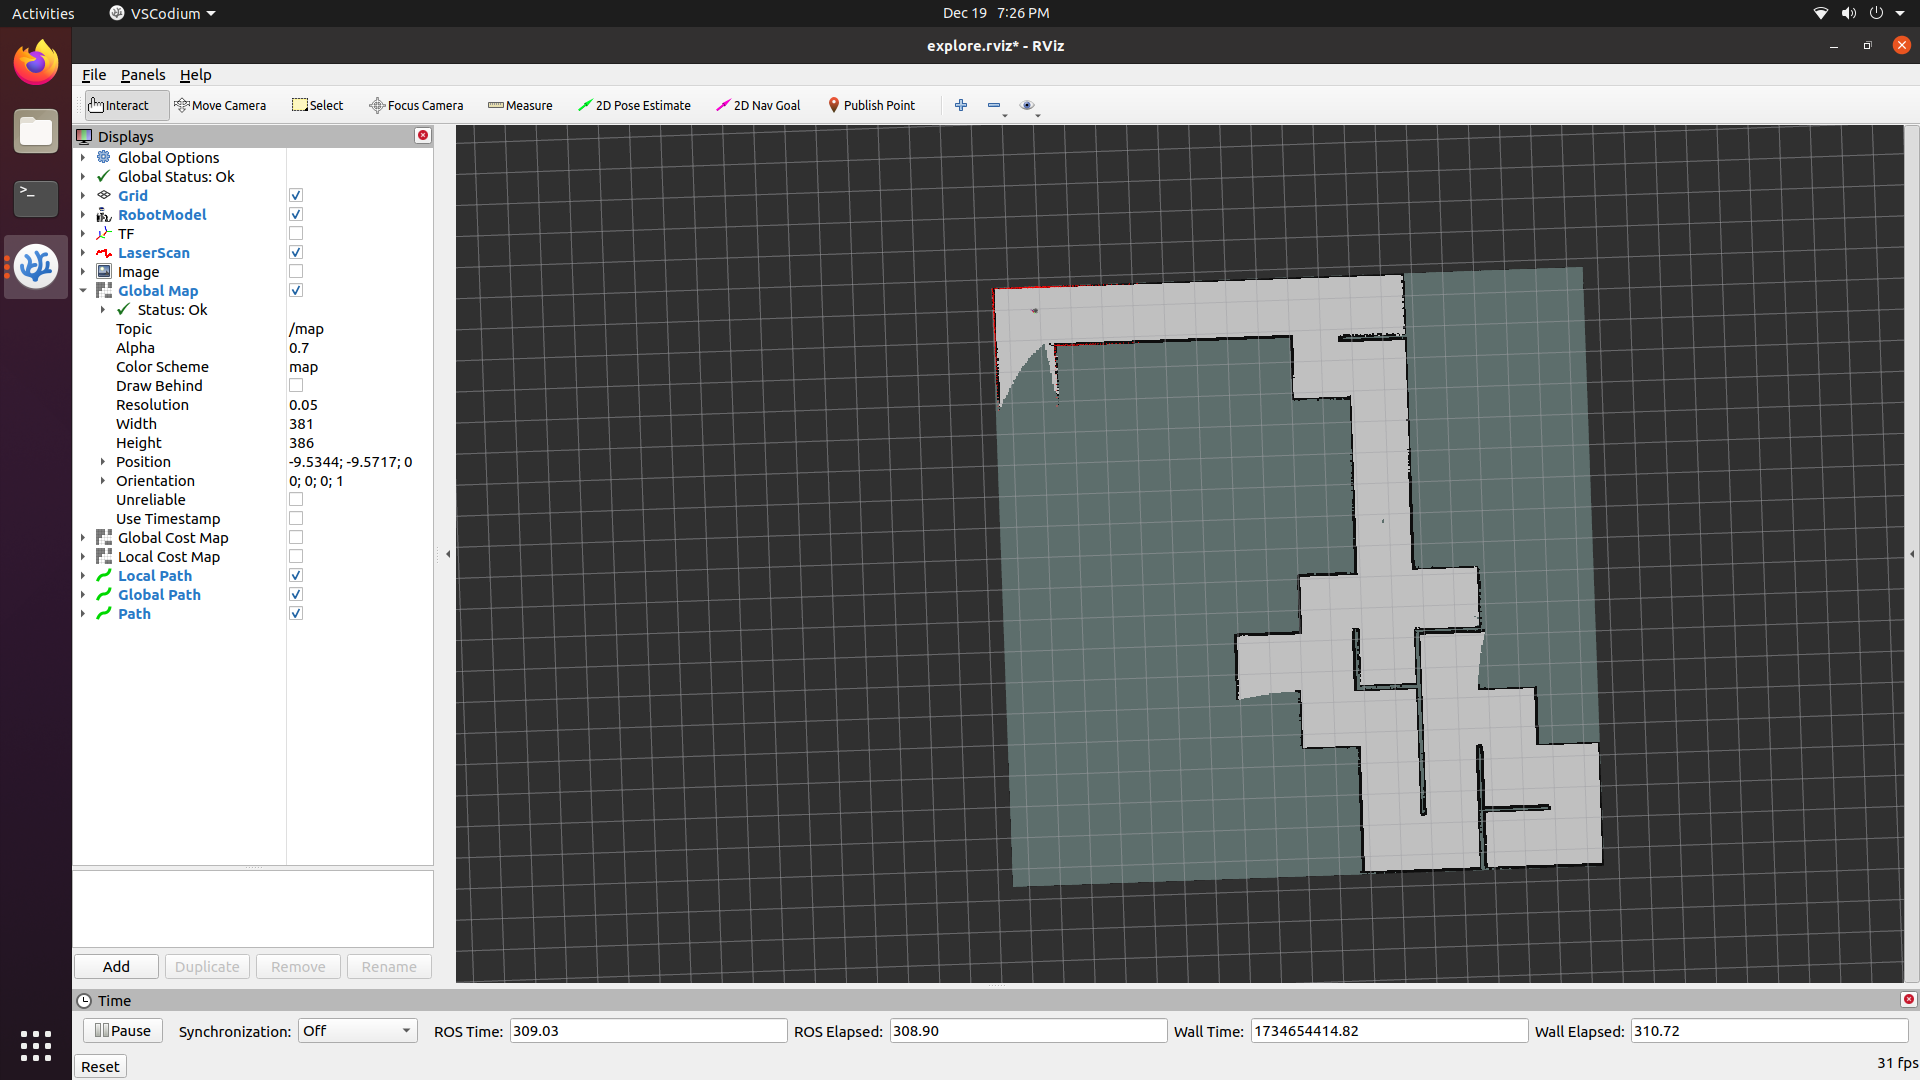
\includegraphics[width=\linewidth]{maze_4_karto.png} 
\end{figure}

{\bf Time it Took to Reach Goal:} \\\\
\begin{tabular}{ |p{3cm}||p{3cm}|p{3cm}|p{3cm}|  }
 \hline
 \multicolumn{4}{|c|}{Time (in minutes, seconds, milliseconds)} \\
 \hline
 Maze & GMapping &Hector & Karto\\
 \hline
 Maze 1   & 1.53.28    &1:53.62&   1:56.12\\
 Maze 3 &  1:33.62  & 1:31.03   &1:32.19\\
 Maze 4  &9:55.05 & 8:33.64&  3:22.78\\
 \hline
\end{tabular}
\\
\\
It is worth noting that the Hector algorithm, while performing well, took multiple tries to work and fine tuning to the parameters of the robot, since it was an algorithm designed for a very specific context. 

\subsection{Analysis of Results}
Maze 1 and Maze 3 all had similar results, meaning that each Turtlebot, guided by its respective algorithm, was able to successfully traverse the maze on its own, even for Karto, when we were guiding it step by step towards the goal, because its sensor measurement is limited and only has a very small view of its surroundings. This can probably be attributed to each maze's simple design, and lack of confounding direction. 

However, Maze 4 demonstrates vastly different times between Gmapping, Hector, and Karto. Gmapping takes the longest, but it is able to successfully navigate by itself to the goal without any help by the user. Hector is a bit more complicated. It tries to navigate to the goal by itself, but gets stuck at this corner of the maze: 
\pagebreak

\begin{figure}[htbp]
    \centering
    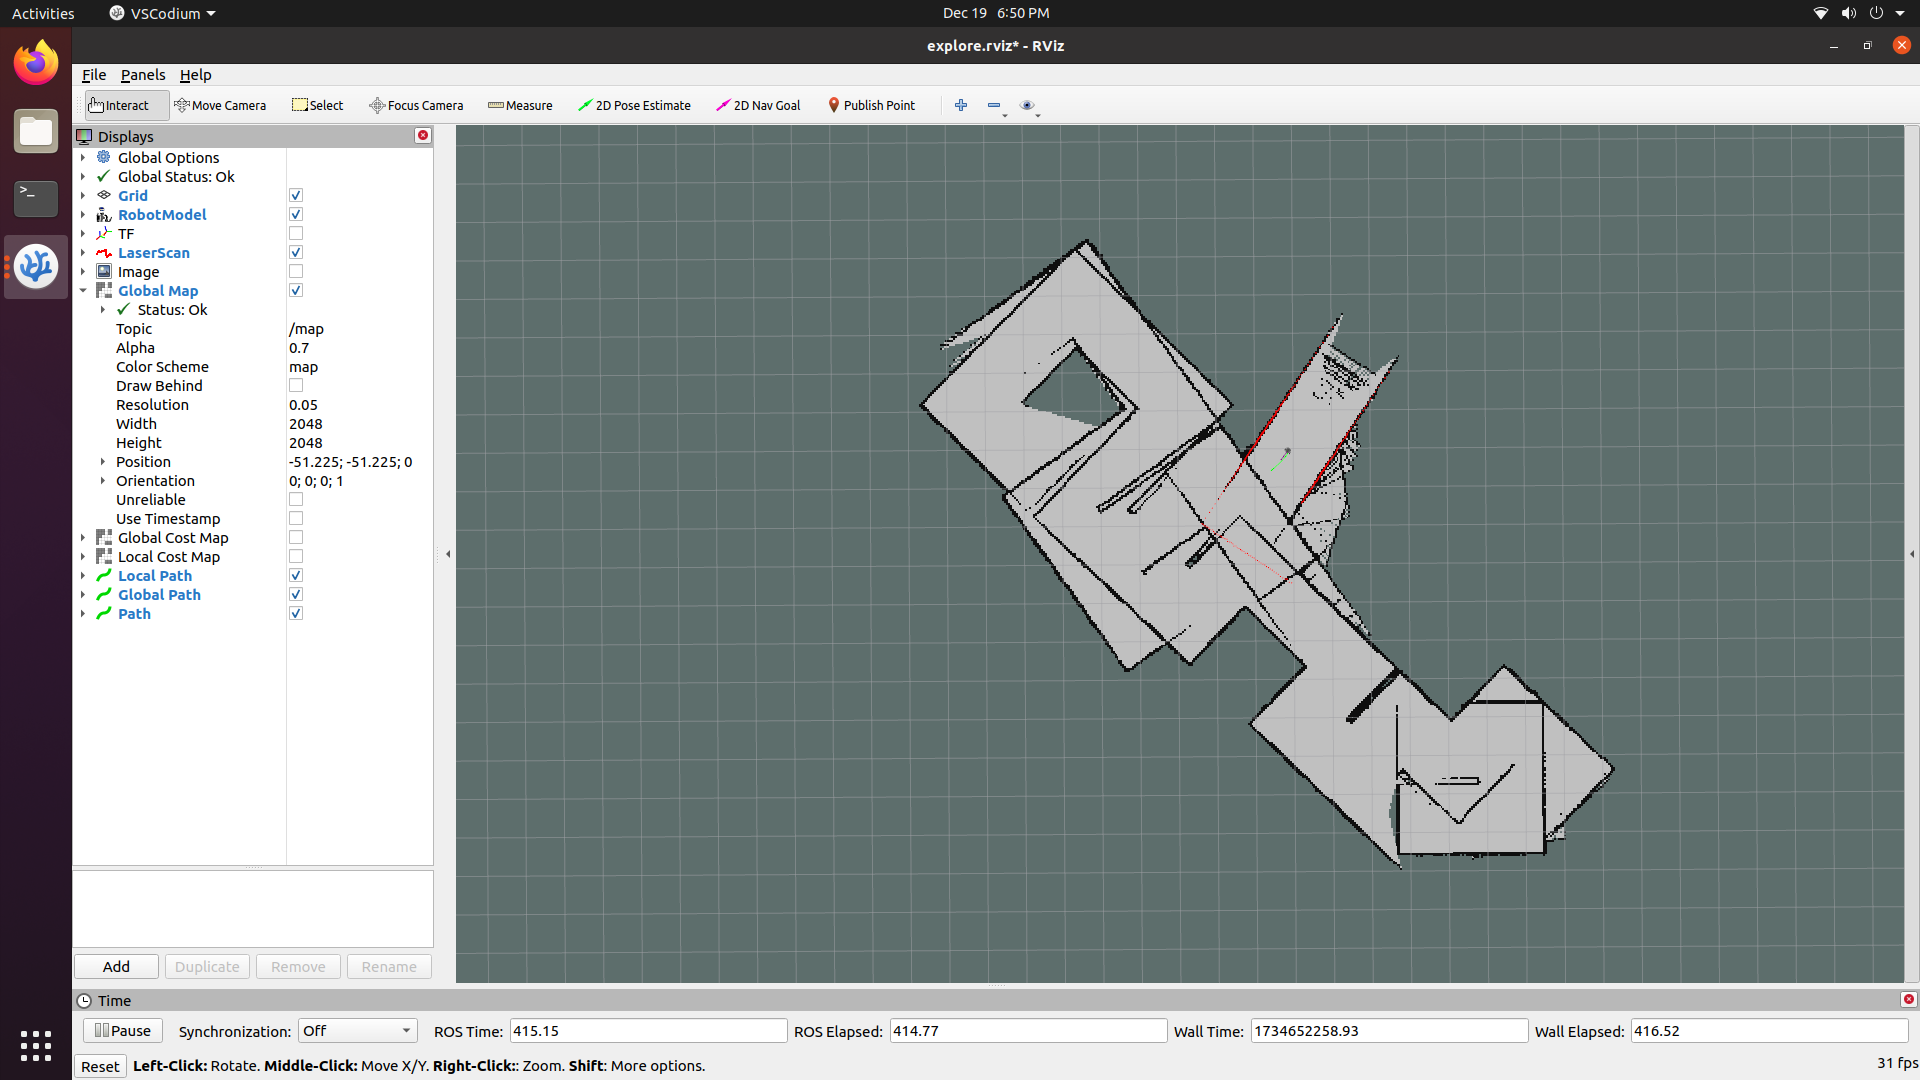
\includegraphics[width=\linewidth]{maze_4_hector_trial_1.png} 
\end{figure}


We had to restart Hector's run through. Finally, on the third run, before it got too stuck in the corner, we guided it to the goal, culminating in the shorter runtime. Karto took the shortest time because of its limited measurement of the world around it, letting the user simply guide it through the maze. 

This experiment demonstrated each algorithm's flaws and strengths well. Gmapping handles large and sparse maps well, perfect for traversing a maze with a wide space, but maybe if the walls were tighter and smaller, its computationally expensive approach with particle filters may fail. While Hector is incredibly precise, when its odometry fails or when there is a large map (like maze 4), it will start to fail. Karto is extremely accurate in large environments, but needs a lot of updates and has a limited worldview, which may not be great in a maze with a lot of features. 


\section{Conclusion and Future Work}

In conclusion, using different SLAM algorithms to traverse a maze highlighted each algorithm's flaws and strengths. Although we used a maze with quite a wide space, to really hone in and deconstruct each algorithm specifically would require making mazes of all different kinds, or adding some other feature, like obstacles, that the Turtlebot would need to avoid. 

For future work, it would be interesting to be able to redo this experiment with a physical robot to see how the simulation differs from real life, and compare the accuracy. The simulation can help form a basis of beliefs for how the different algorithms can perform for both path-finding and SLAM. Additionally, more dynamic environments can be used to further test the algorithms in different scenarios to see which is best for each task. Hopefully, a team can take on these experiments to further improve a robot's path-finding, localization, and/or mapping abilities, which will make it even more useful and efficient in aiding humans in certain tasks, or open up new applications of these techniques and algorithms in the field. 

\bibliographystyle{plain}
\begin{thebibliography}{9}


\bibitem{Yarovoi2024}
A. Yarovoi and Y. K. Cho, ``Review of simultaneous localization and mapping (SLAM) for construction robotics applications,'' Automation in Construction, vol. 162, pp. 105344, 2024, doi: 10.1016/j.autcon.2024.105344.

\bibitem{Thale2020}
S. P. Thale, M. M. Prabhu, P. V. Thakur, P. Kadam, ``ROS based SLAM implementation for Autonomous navigation using Turtlebot,'' ITM Web Conf., vol. 32, pp. 01011, 2020, doi: 10.1051/itmconf/20203201011.

\bibitem{Abiyev2017}
R. H. Abiyev, M. Arslan, I. Gunsel, and A. Cagman, ``Robot Pathfinding Using Vision Based Obstacle Detection,'' in Proc. 2017 3rd IEEE International Conference on Cybernetics (CYBCONF), Exeter, UK, 2017, pp. 1-6, doi: 10.1109/CYBConf.2017.7985805.

\bibitem{Turnage2016}
D. M. Turnage, ``Simulation results for localization and mapping algorithms,'' in Proc. 2016 Winter Simulation Conference (WSC), Washington, DC, USA, 2016, pp. 3040-3051, doi: 10.1109/WSC.2016.7822338.

\bibitem{Cherubini2014}
A. Cherubini, F. Spindler, and F. Chaumette, ``Autonomous Visual Navigation and Laser-Based Moving Obstacle Avoidance,'' IEEE Transactions on Intelligent Transportation Systems, vol. 15, no. 5, pp. 2101-2110, Oct. 2014, doi: 10.1109/TITS.2014.2308977.

\bibitem{Sang2024}
W. Sang, Y. Yue, K. Zhai, and M. Lin,  ``Research on AGV Path Planning Integrating an Improved A* Algorithm and DWA Algorithm,'' Applied Sciences, vol. 14, no. 17, p. 7551, 2024, doi: 10.3390/app14177551.

\bibitem{Lai2023}
X. Lai, et al., ``Enhanced DWA Algorithm for Local Path Planning of Mobile Robot,'' The Industrial Robot, vol. 50, no. 1, pp. 186-194, 2023. 


\end{thebibliography}


\end{document}
